% !TeX root = main.tex

\appendix
\section*{Annexes}
\addcontentsline{toc}{section}{Annexes}

% ---------------------------------------------------------------------

% ---------------------------------------------------------------------

% ---------------------------------------------------------------------

% ---------------------------------------------------------------------

% ---------------------------------------------------------------------
\subsection*{Annexe A - Textes réglementaires de référence}
\addcontentsline{toc}{subsection}{Annexe A - Textes réglementaires}
\label{ann:textes_loi}

Les différents textes juridique la profession de géomètre-expert, cités dans ce mémoire, sont consultables intégralement sur le portail Légifrance :

\begin{itemize}
  \item Loi n°46-942 du 7 mai 1946 instituant l'Ordre des géomètres-experts :\\
  \url{https://www.legifrance.gouv.fr/loi/id/LEGITEXT000006068236/}

  \item Décret n°96-478 du 31 mai 1996 portant règlement de la profession de géomètre-expert et code des devoirs professionnels :\\
  \url{https://www.legifrance.gouv.fr/legi/id/LEGIARTI000006842596/}
\end{itemize}

L'article 55 du décret de 1996, relatif à l'obligation de conservation des archives, est directement accessible via :
\begin{center}
  \url{https://www.legifrance.gouv.fr/legi/article/LEGIARTI000006842596}
\end{center}

\clearpage

% ---------------------------------------------------------------------
\subsection*{Annexe B - Architecture du modèle LayoutLM}
\addcontentsline{toc}{subsection}{Annexe B - Architecture de LayoutLM}
\label{ann:layoutlm}

\begin{figure}[H] 
  \centering
  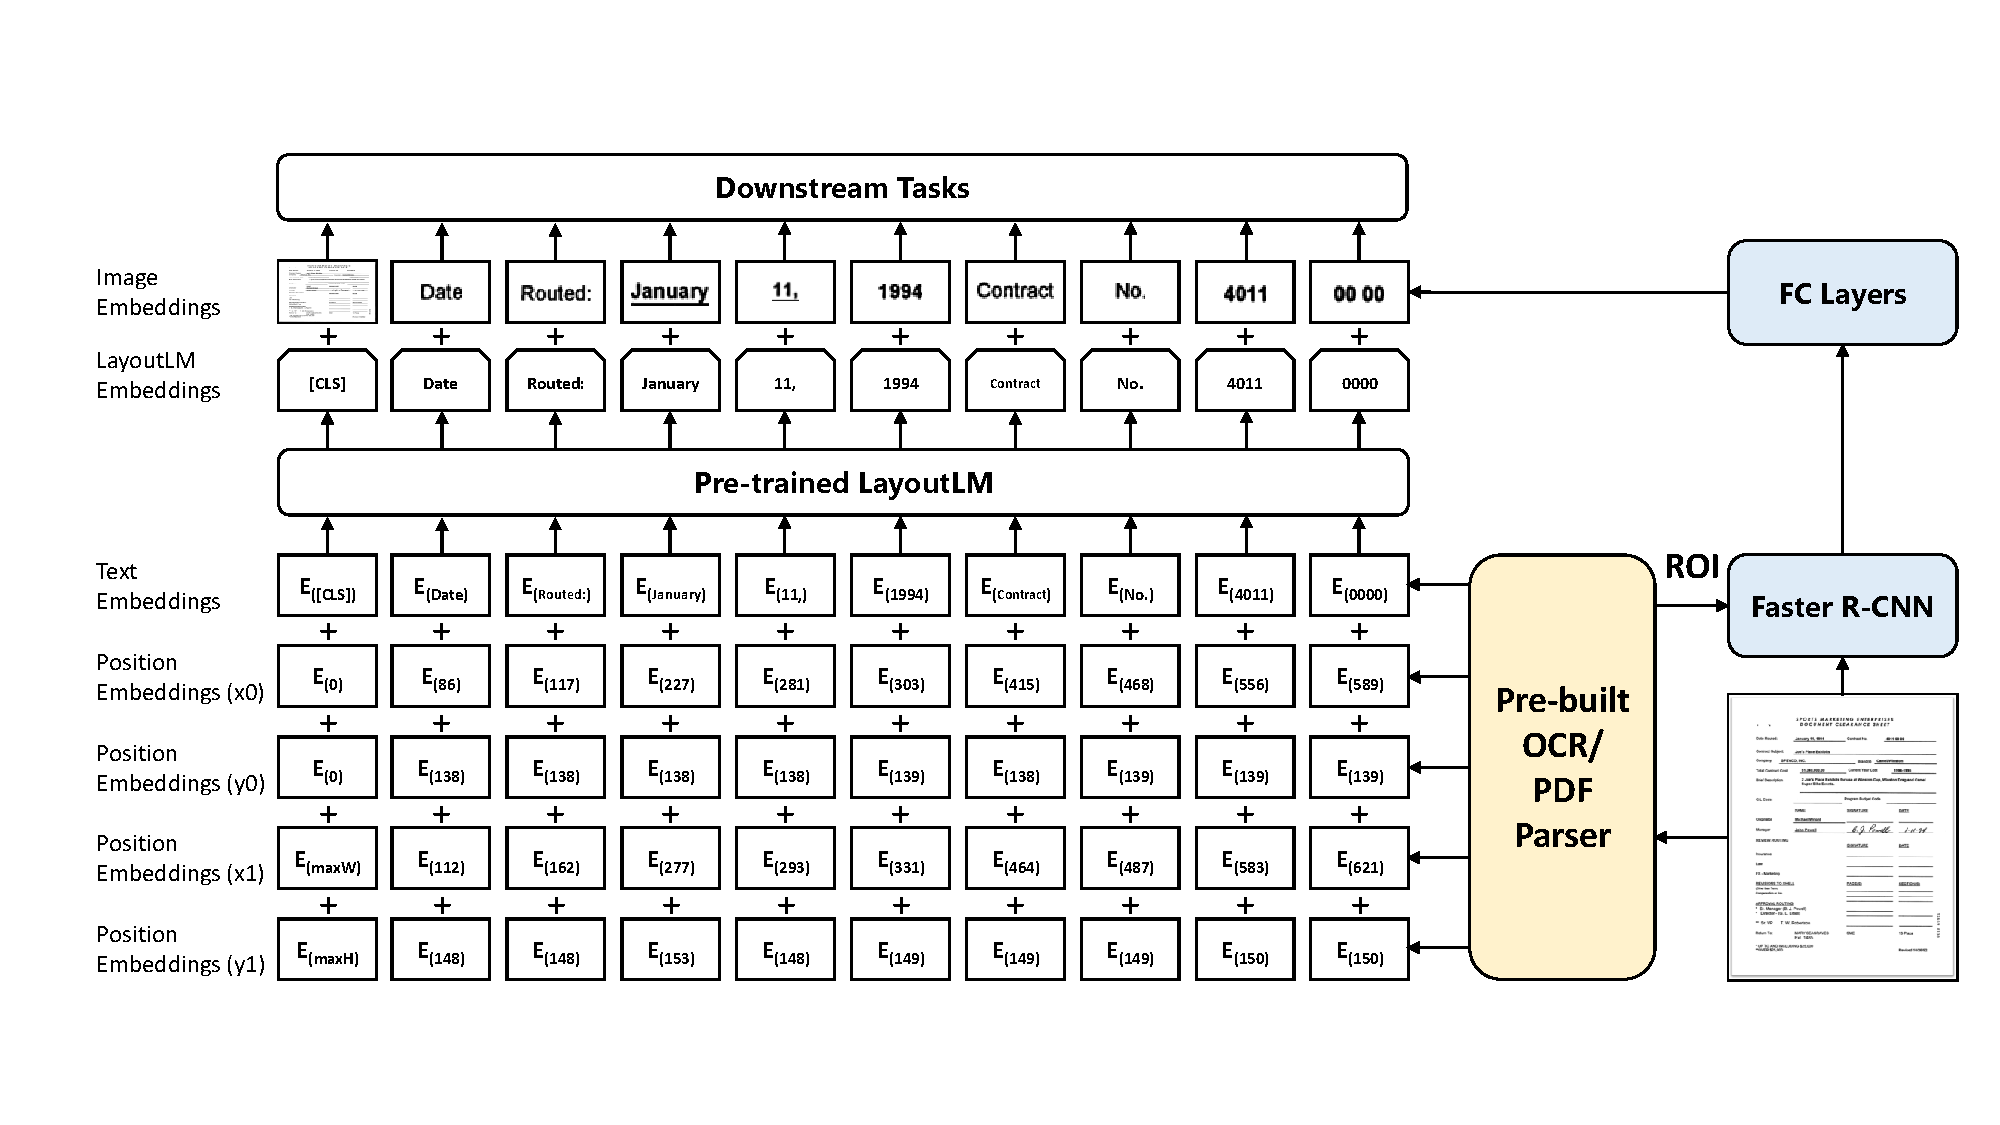
\includegraphics[width=0.80\textheight, angle=90]{img/layoutlm_arch.pdf}
  \caption*{Architecture du modèle multimodal LayoutLM (présentée en grand format horizontal). Extrait de \cite{xu_layoutlm_2020}.}
  \label{fig:layoutlm_annexe}
\end{figure}

\clearpage
% ---------------------------------------------------------------------
\subsection*{Annexe C - Matrice de confusion du modèle LayoutLM}
\addcontentsline{toc}{subsection}{Annexe C - Matrice de confusion de LayoutLM}
\label{ann:layoutlm_confusion}

\begin{figure}[H]
  \centering
  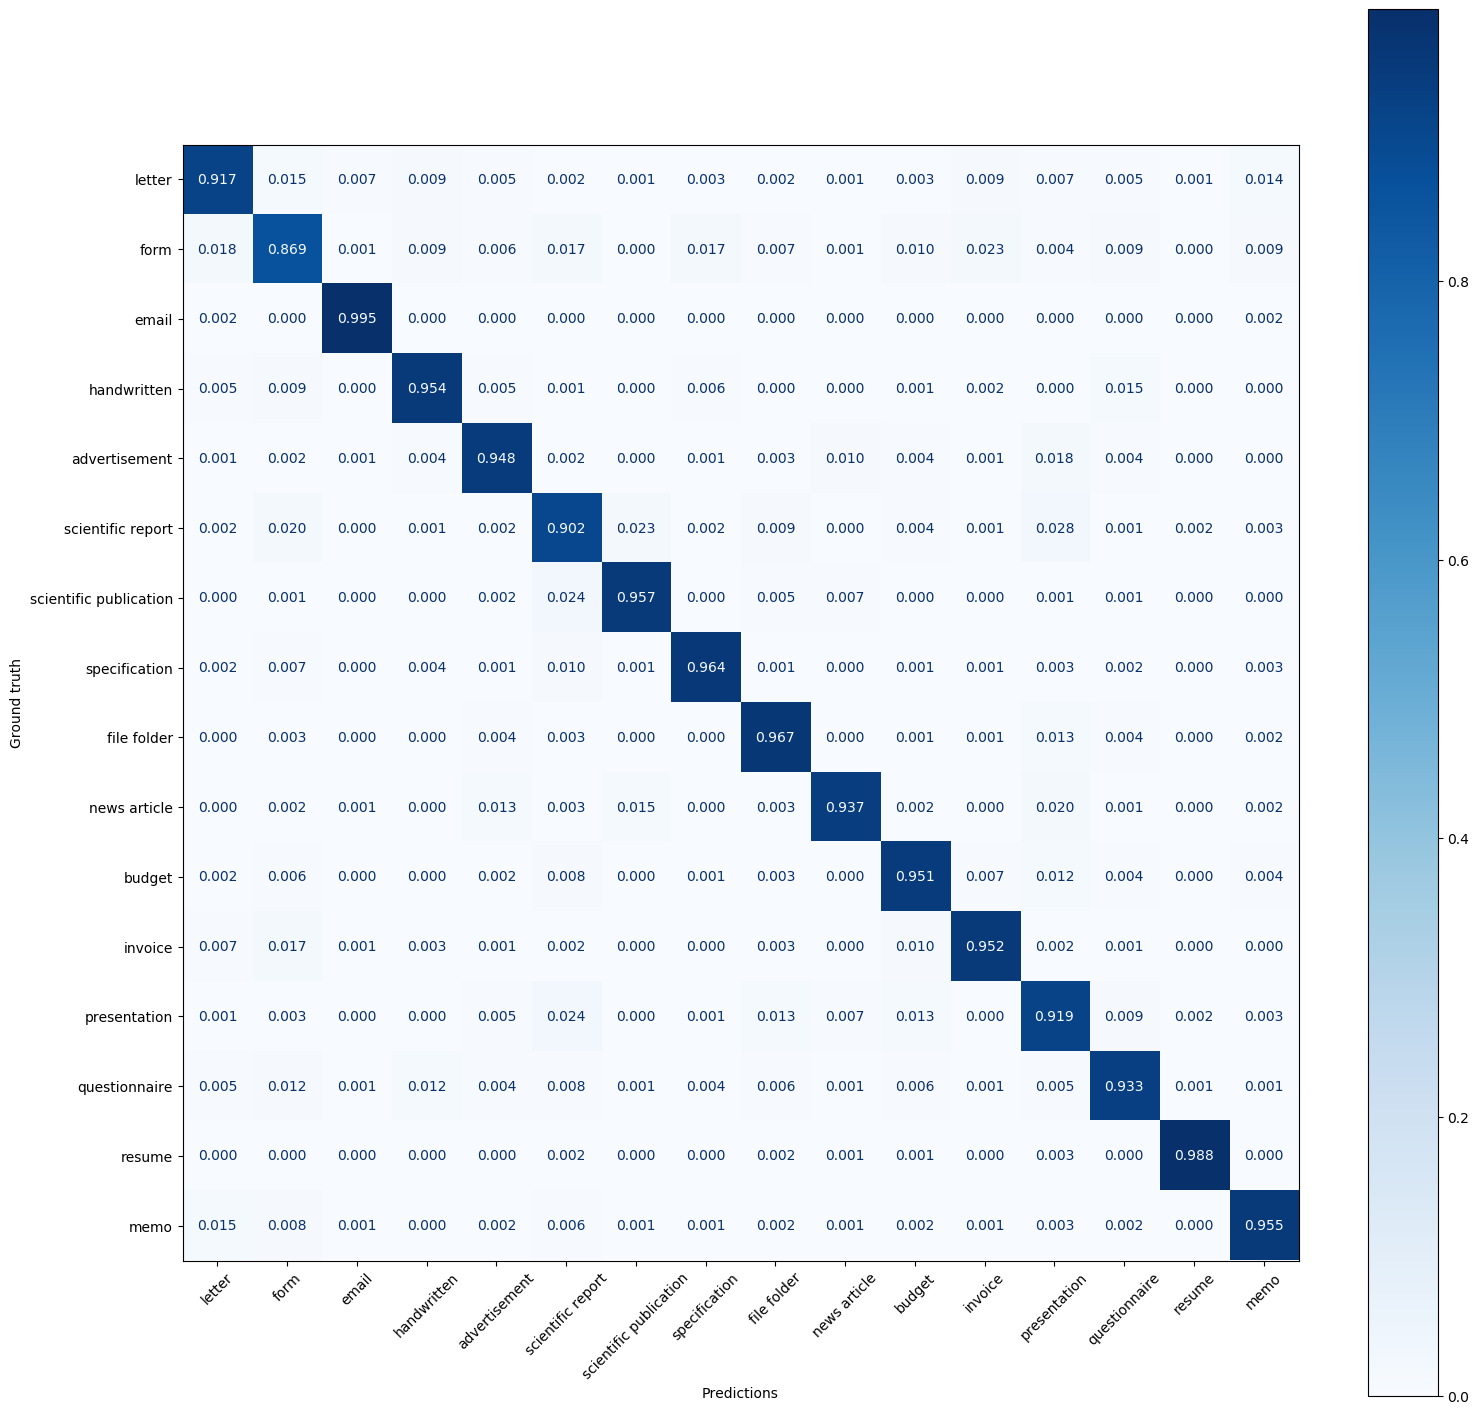
\includegraphics[width=0.80\textheight, angle=90]{img/layoutlm_confusion.png}
  \caption*{Matrice de confusion du modèle LayoutLM (présentée en grand format horizontal). Extrait de \cite{xu_layoutlm_2020}.}
  \label{fig:layoutlm_confusion_annexe}
\end{figure}

\clearpage

% ---------------------------------------------------------------------
\subsection*{Annexe D - Architecture globale du modèle GLiNER}
\addcontentsline{toc}{subsection}{Annexe D - Architecture de GLiNER}
\label{ann:gliner_architecture}

\begin{figure}[H]
  \centering
  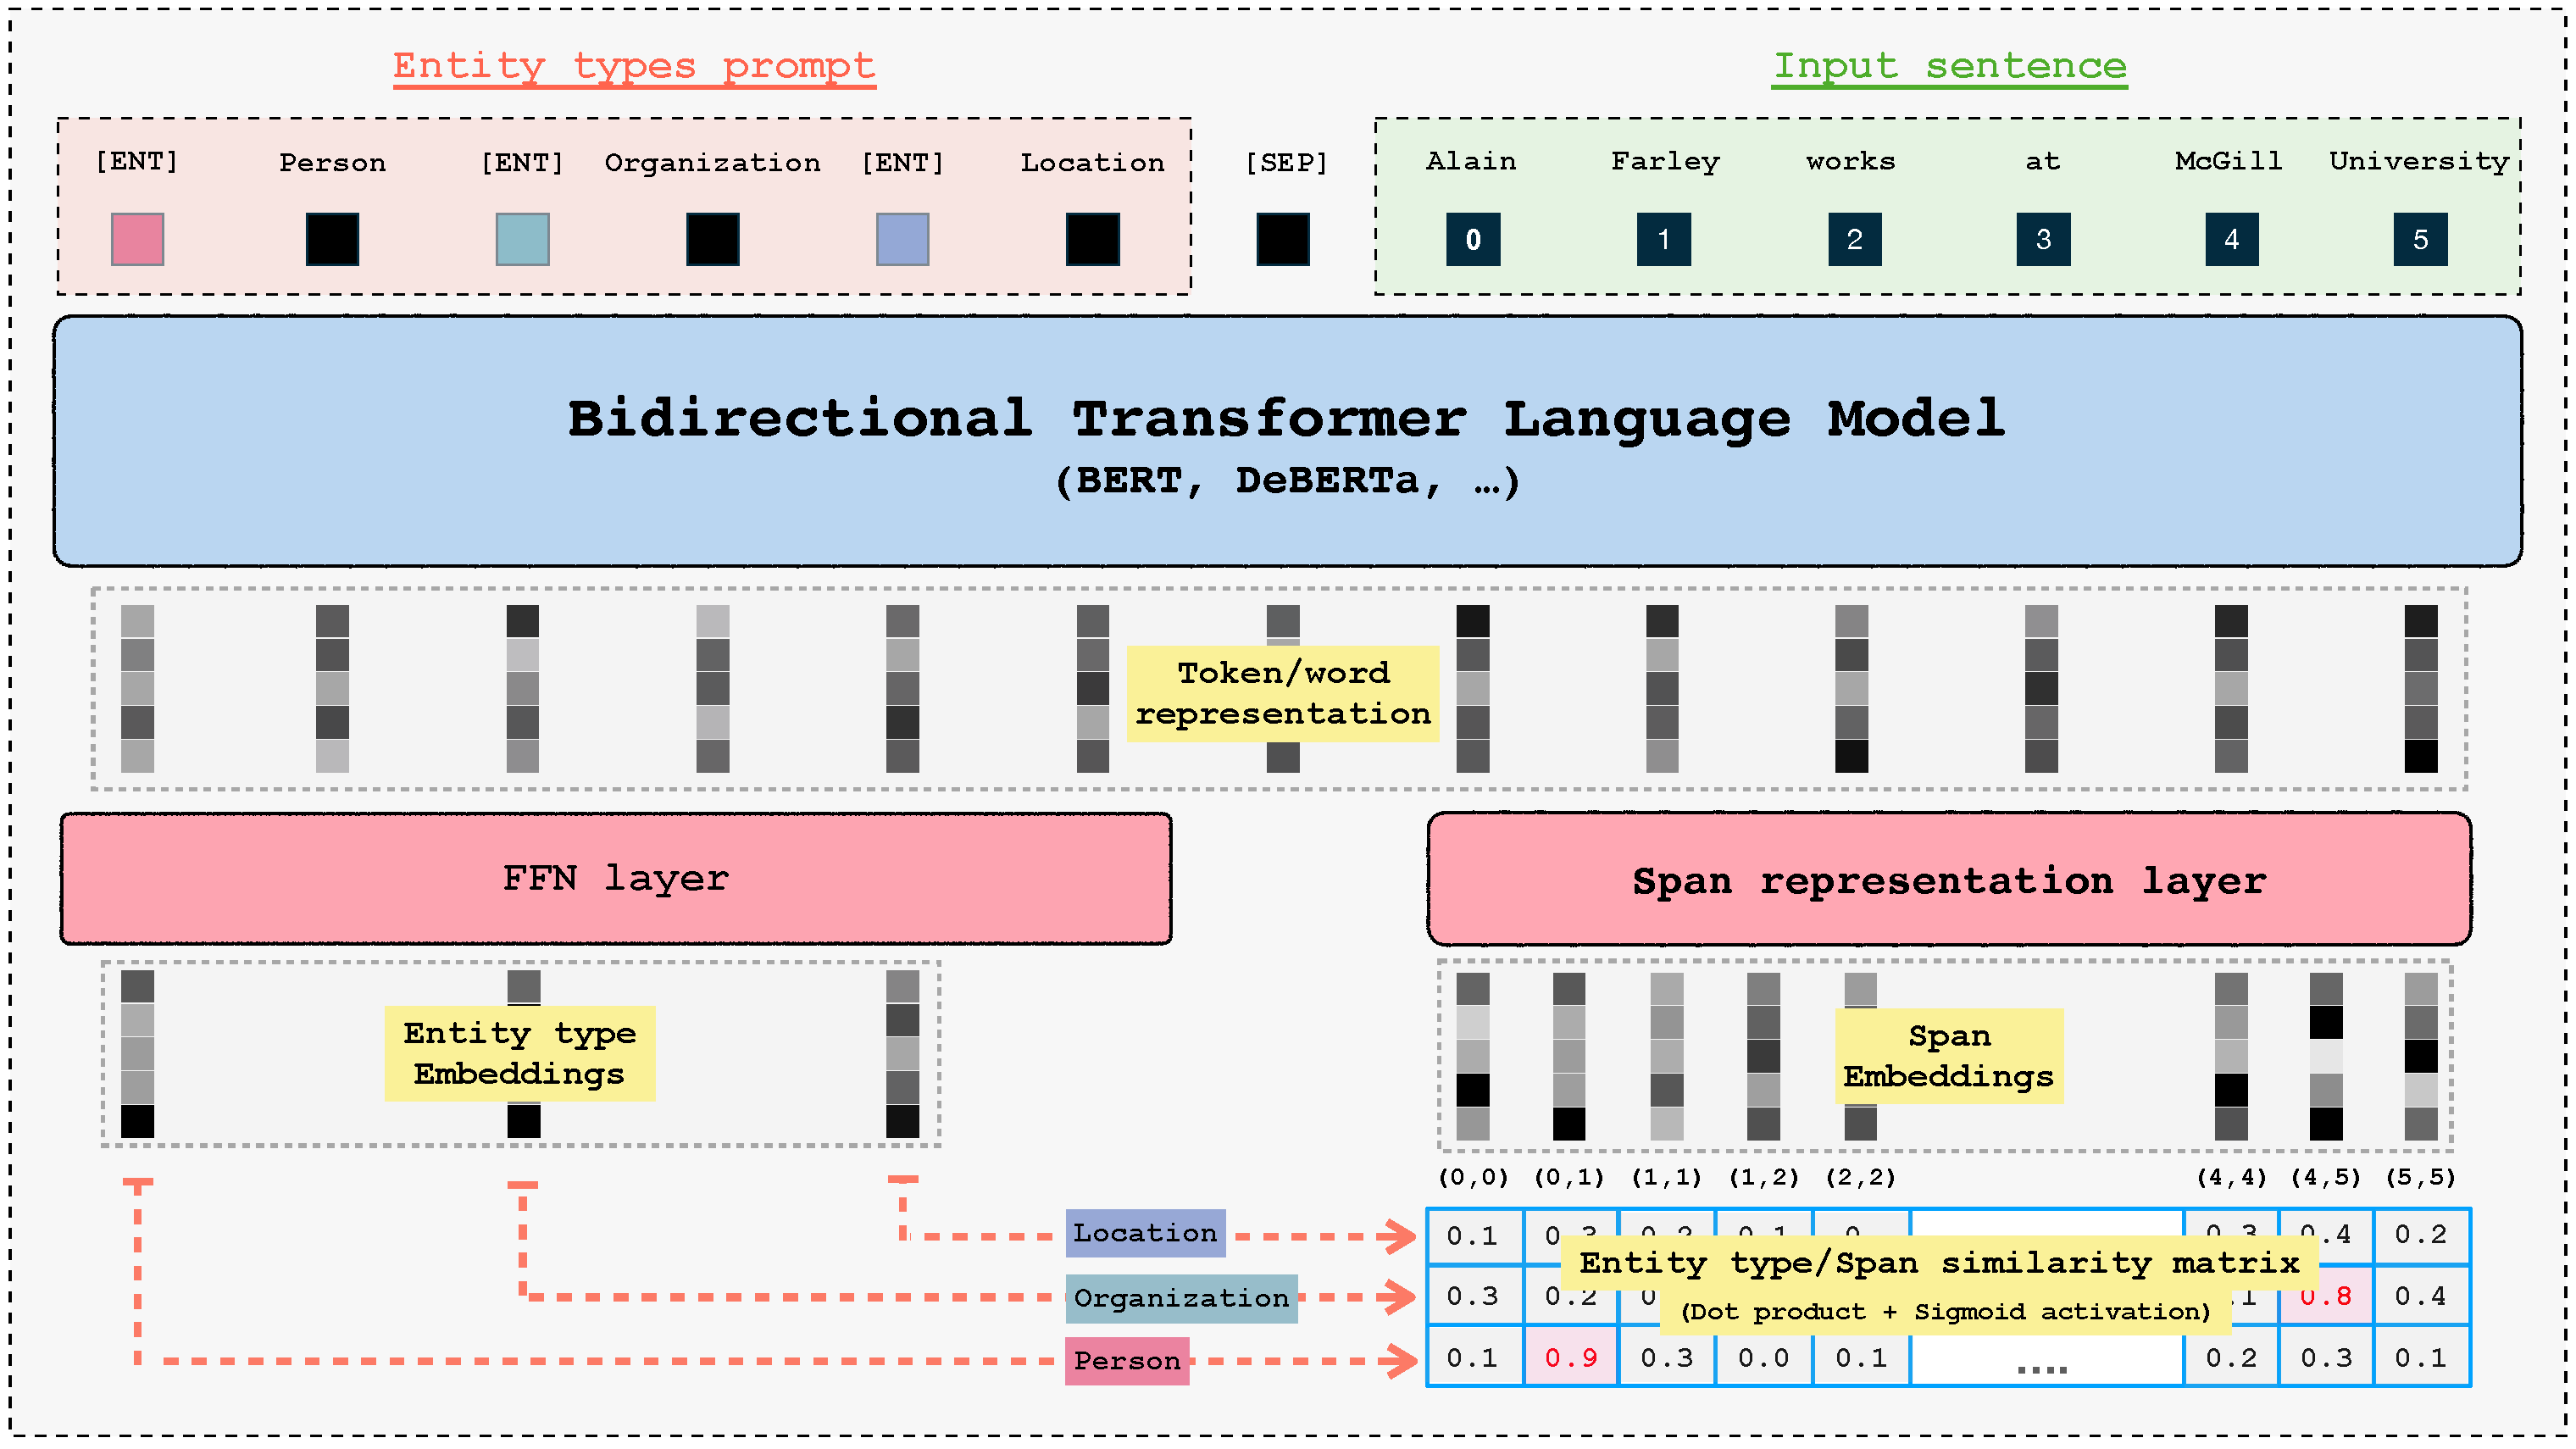
\includegraphics[width=0.80\textheight, angle=90]{img/gliner_gener.pdf}
  \caption*{Architecture globale du modèle GLiNER (présentée en grand format horizontal). Extrait de \cite{zaratiana_gliner_2024}.}
  \label{fig:gliner_annexe}
\end{figure}

\clearpage

% ---------------------------------------------------------------------
\subsection*{Annexe E - Architecture du modèle Vision-Langage LLaVA}
\addcontentsline{toc}{subsection}{Annexe E - Architecture de LLaVA}
\label{ann:llava_architecture}

\begin{figure}[H]
  \centering
  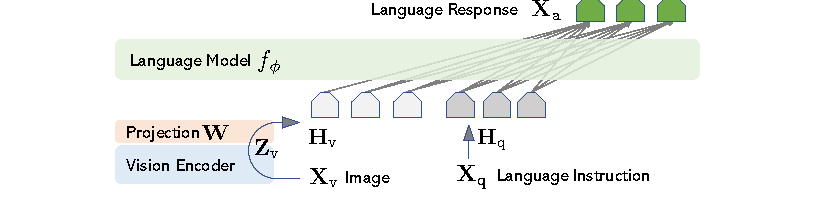
\includegraphics[width=0.80\textheight, angle=90]{img/llava_arch.pdf}
  \caption*{Architecture interne du modèle Vision-Langage LLaVA (présentée en grand format horizontal). Extrait de \cite{liu_llava_2024}.}
  \label{fig:llava_annexe}
\end{figure}

\clearpage

% ---------------------------------------------------------------------
\subsection*{Annexe F - Interface de validation du répertoire du Géomètre A}
\addcontentsline{toc}{subsection}{Annexe F - Interface du Géomètre A}
\label{ann:interface_geometre_a}

\begin{figure}[H]
  \centering
  \setlength{\fboxsep}{0pt}%
  \setlength{\fboxrule}{0.6pt}%
  \fbox{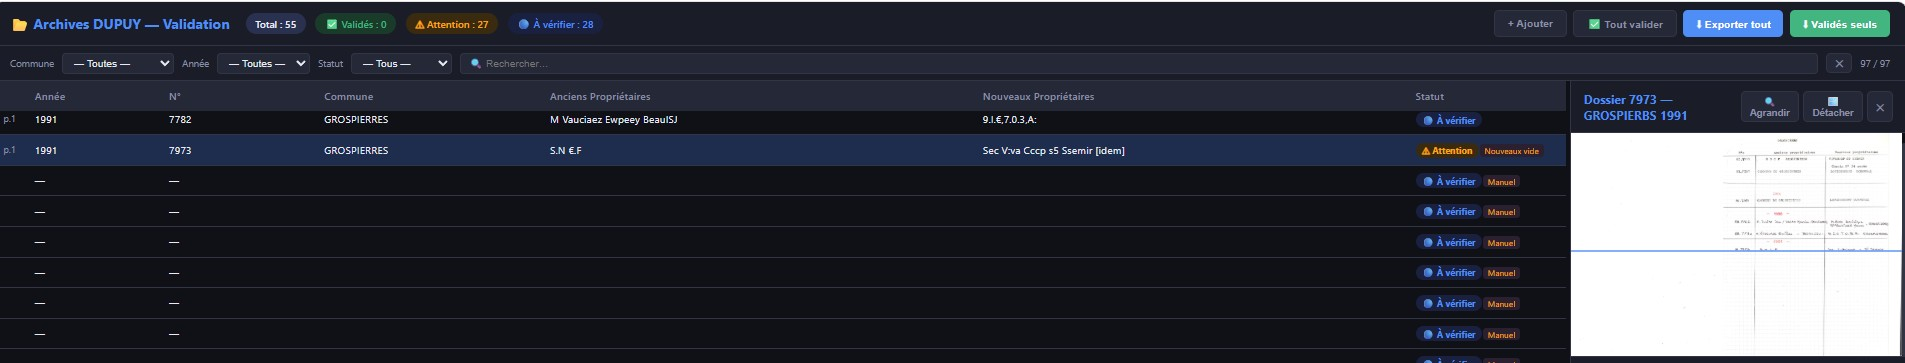
\includegraphics[width=0.94\textheight, keepaspectratio, angle=90]{img/5.5_reprtoire_A_liste.jpg}}
  \label{fig:interface_geometre_a_liste_annexe}
\end{figure}

\clearpage

\begin{figure}[H]
  \centering
  \setlength{\fboxsep}{0pt}%
  \setlength{\fboxrule}{0.6pt}%
  \fbox{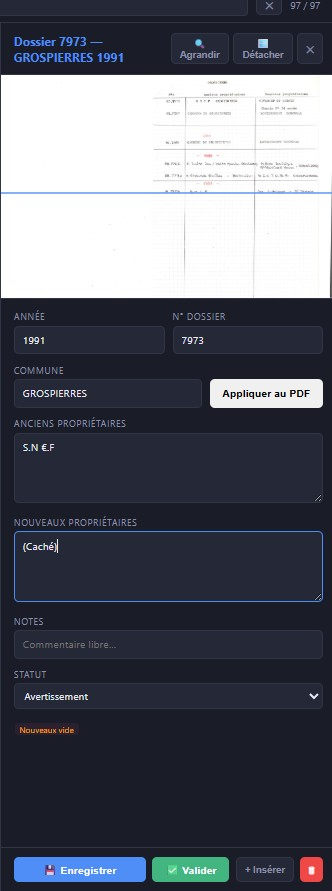
\includegraphics[height=0.82\textheight, keepaspectratio]{img/5.5_reprtoire_A_infos.jpg}}
  \caption*{Interface de validation du répertoire du Géomètre A (port 5050) -- Fiche détaillée et édition des champs (grand format).}
  \label{fig:interface_geometre_a_infos_annexe}
\end{figure}



